\chapter{フリードマン力学：物質、放射、真空エネルギー}

\lectureoverview{膨張宇宙の運動学は一行で述べることができる。すなわち、物理的な距離はスケール因子\(a(t)\)とともに増大する。問題は今や、その関数を決定することである。我々は平坦空間のフリードマン方程式をニュートン的なエネルギー保存から導き、まず通常の物質について解き、次に放射と真空エネルギーがなぜ全く異なる宇宙の歴史をもたらすのかを見るであろう。}

\section{説明されるべき幾何学}

固定された宇宙時刻において、大規模な宇宙は一様かつ等方に見える。銀河、銀河団、超銀河団は確かに実在する構造であるが、数億光年あるいは数十億光年のスケールでは、その分布は驚くほど一様になる。この経験的な規則性は宇宙原理と呼ばれる。その名がこれを定理にするわけではない。この原理の力は観測から来るのである。

第二の経験的事実がある。現在の精度の範囲内では、大きな空間的三角形はユークリッド三角形として振る舞う。サッカー場を測量することとの比較が有用である。ぴんと張った線がなす三角形の角の和が\(180^\circ\)になるとしても、それによって地球が大域的には平坦であることが証明されたわけではない。示されたのは、地球の曲率半径がサッカー場に比べて大きいということである。宇宙の測量も同じ論理形式をもつ。空間は非常に大きな曲率半径をもつかもしれないが、観測可能な領域では平坦であるとよく近似される。

基準となる幾何学はミンコフスキー時空であり、
\begin{equation}
  d\tau^2=dt^2-\left(dx^2+dy^2+dz^2\right).
  \label{eq:l09-minkowski}
\end{equation}
括弧は三次元におけるユークリッド距離要素にほかならない。これに対して一般相対性理論では、座標微分の係数は場である。それらは位置と時間によって変化し得るし、混合項も現れ得る。これらの計量係数は、ニュートン的重力場の相対論的な後継者である。

\begin{figure}[H]
  \centering
  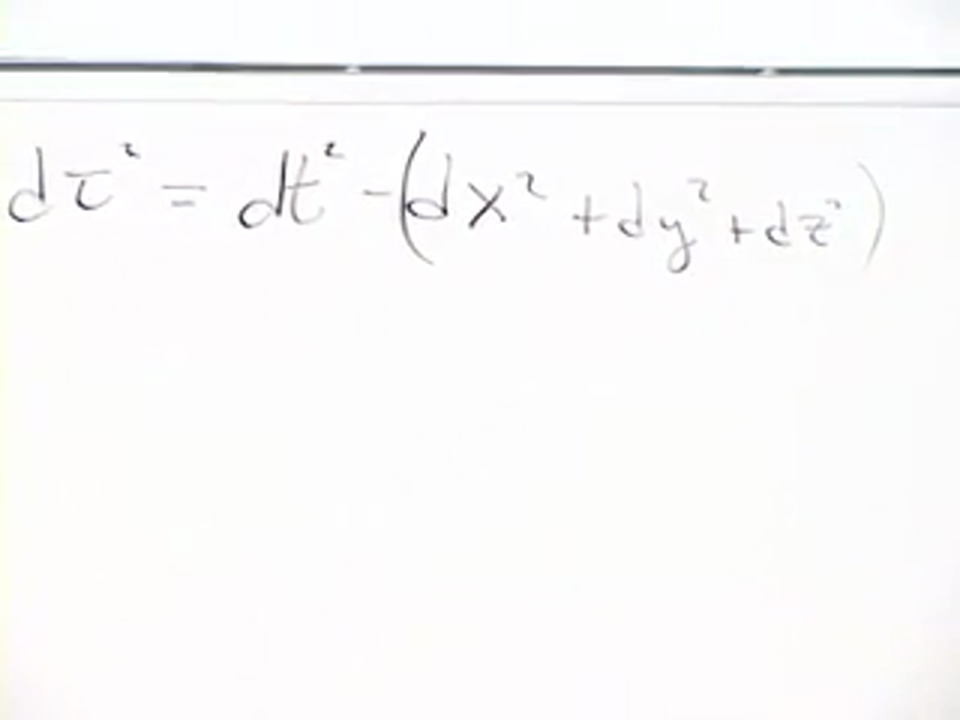
\includegraphics[width=0.72\textwidth]{lecture_09_figure_01.png}
  \caption{講義の冒頭で書かれたミンコフスキー固有時間要素。00時01分50秒のソースフレーム。}
  \label{fig:l09-minkowski-board}
\end{figure}

空間的に平坦な膨張宇宙では、一様性と等方性により、時間に依存する一つのスケール因子が残る：
\begin{equation}
  d\tau^2=dt^2-a^2(t)\left(dx^2+dy^2+dz^2\right).
  \label{eq:l09-flat-frw}
\end{equation}
我々は\(c=1\)とする単位系を用いるので、時間と長さは同じ次元をもつ。整合的な二つの規約がある。\(x,y,z\)に長さの次元を与え、\(a\)を無次元とみなすこともできるし、\(x,y,z\)を無次元のラベルとして扱い、\(a\)に長さの次元をもたせることもできる。本講義では第二の規約を用いる。それは\(a(t)\)の物理的意味を可視化するからである。

\begin{figure}[H]
  \centering
  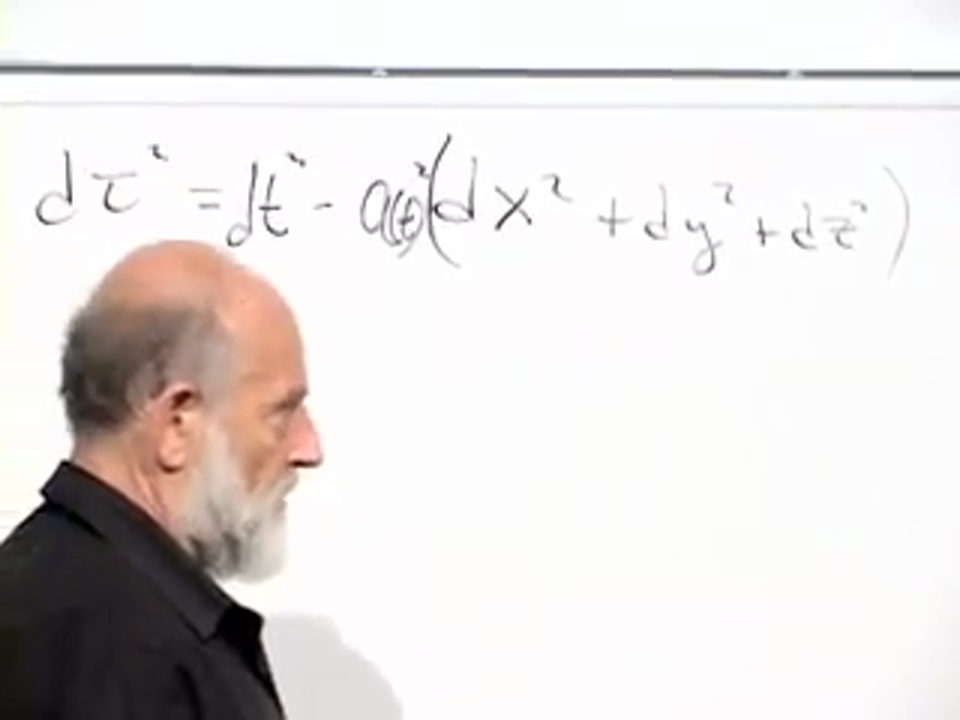
\includegraphics[width=0.72\textwidth]{lecture_09_figure_02.png}
  \caption{平坦な膨張計量であり、スケール因子がユークリッド空間的線要素に掛かる。00時09分12秒のソースフレーム。}
  \label{fig:l09-expanding-metric-board}
\end{figure}

ゴムのシートに座標が描かれていると想像しよう。座標の印はシートに貼り付いたままであるが、それらの間の物理的距離は増大する。したがって、「\(x=0\)から\(x=1\)まで」といった座標の差は、単なる一対のラベルにすぎない。その区間が表す距離は\(a(t)\)である。このスケール因子を支配する方程式を見出すことが、本講義の力学の問題である。

\section{閉じた、平坦な、開いた空間幾何学}

平坦性は観測上の単純化であり、一様性の帰結ではない。一様かつ等方な空間幾何学は三つある。正の曲率、零の曲率、負の曲率である。正の場合を理解するには、次元について正確であることが助けになる。

軌跡
\begin{equation}
  X_1^2+X_2^2=R^2
\end{equation}
は円、すなわち一次元球面\(S^1\)である。その内部を埋めたものは円板であり、二次元球体とも呼ばれる。埋め込み座標を一つ加えると
\begin{equation}
  X_1^2+X_2^2+X_3^2=R^2,
\end{equation}
通常の二次元球面\(S^2\)となる。四番目の埋め込み座標を加えると
\begin{equation}
  X_1^2+X_2^2+X_3^2+X_4^2=R^2,
  \label{eq:l09-three-sphere}
\end{equation}
三次元球面\(S^3\)となり、それ自体が三次元空間である。その四次元埋め込みを思い描くことはできないが、内在的幾何学が存在するためにその埋め込みを必要とするわけではない。

\begin{figure}[H]
  \centering
  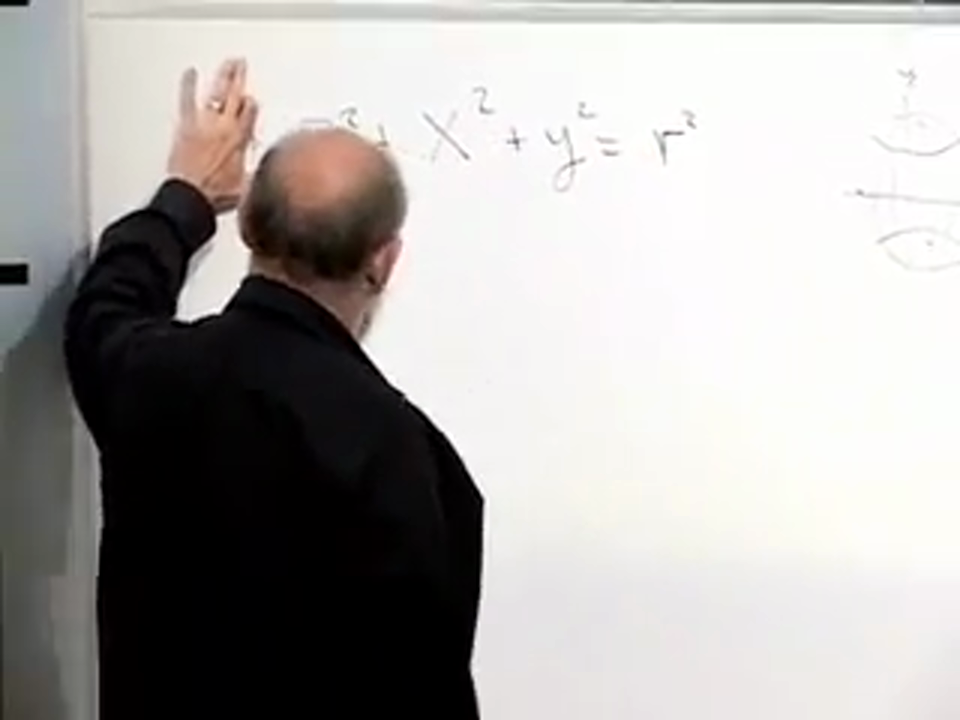
\includegraphics[width=0.72\textwidth]{lecture_09_figure_03.png}
  \caption{三次元球面を導入するために用いられた埋め込み方程式。00時16分40秒のソースフレーム。}
  \label{fig:l09-three-sphere-board}
\end{figure}

理想的な球面のどの点も他のどの点とも幾何学的に等価であり、ある点におけるどの方向も等価である。したがって球面は一様かつ等方の両方である。その半径を\(a(t)\)倍すると、空間全体が、球面上に中心を選ぶことなく膨張または収縮する。そのような宇宙を過去にたどっても、すべての物質が外部の空虚の中の一つの特別な位置に置かれるわけではない。空間全体が小さくなるので、どの点の対も近くなる。ビッグバンは空間のある一点からの爆発ではない。

正に曲がった球面上では、測地線三角形の内角の和は\(180^\circ\)より大きい。平坦な三角形の内角の和はちょうど\(180^\circ\)である。鞍面によって不完全に表される等質な負の曲率をもつ幾何学では、内角の和は\(180^\circ\)より小さい。これらの内在的テストが三つの場合を区別する。

\begin{figure}[H]
  \centering
  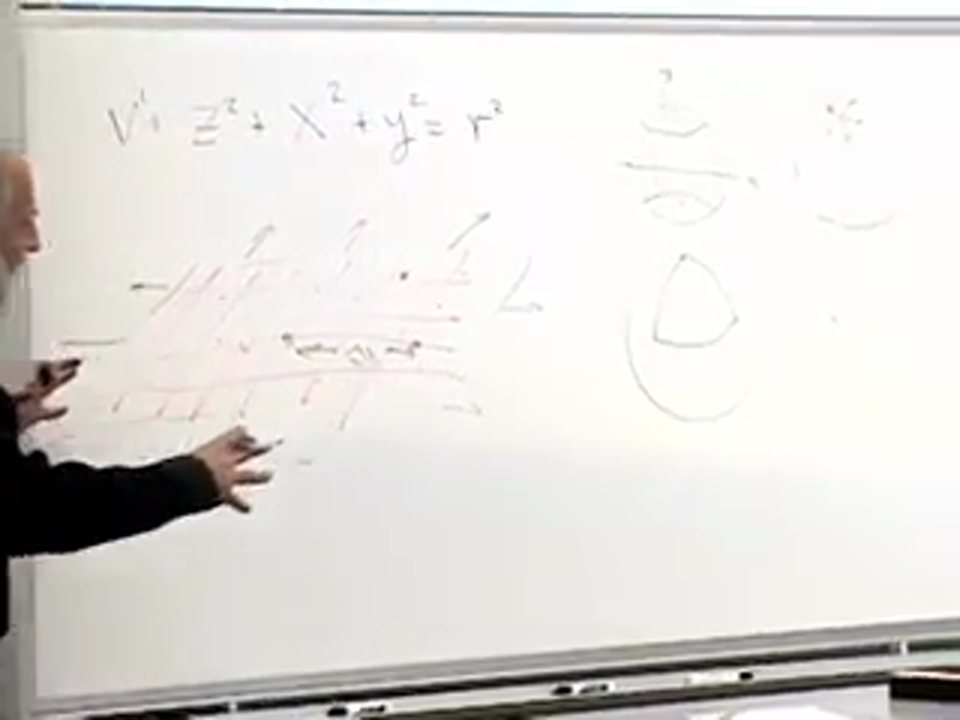
\includegraphics[width=0.72\textwidth]{lecture_09_figure_07.png}
  \caption{正、零、負の曲率をそれぞれの特徴的な三角形の形によって描いたもの。00:37:30のソースフレーム。}
  \label{fig:l09-curvature-board}
\end{figure}

完全に平坦な局所計量は、それ自体では空間が位相的に無限であることを証明しない。コンパクトな平坦位相は数学的に可能であるが、この講義では最も単純な無限ユークリッド模型を採用する。\editorialnote{この大域的位相に関する但し書きは、以降の局所的な力学のいずれにも必要ではない。}

\section{共動ラベルとハッブルの法則}

ここで膨張する平坦なシートに戻り、その上に座標格子を描こう。共動座標では、格子は大規模な物質の流れとともに膨張する。銀河、より正確には十分に粗視化された銀河団は、別の共動物体からの物理的距離が変化しても、ほぼ固定された座標ラベルを保つ。

\begin{figure}[H]
  \centering
  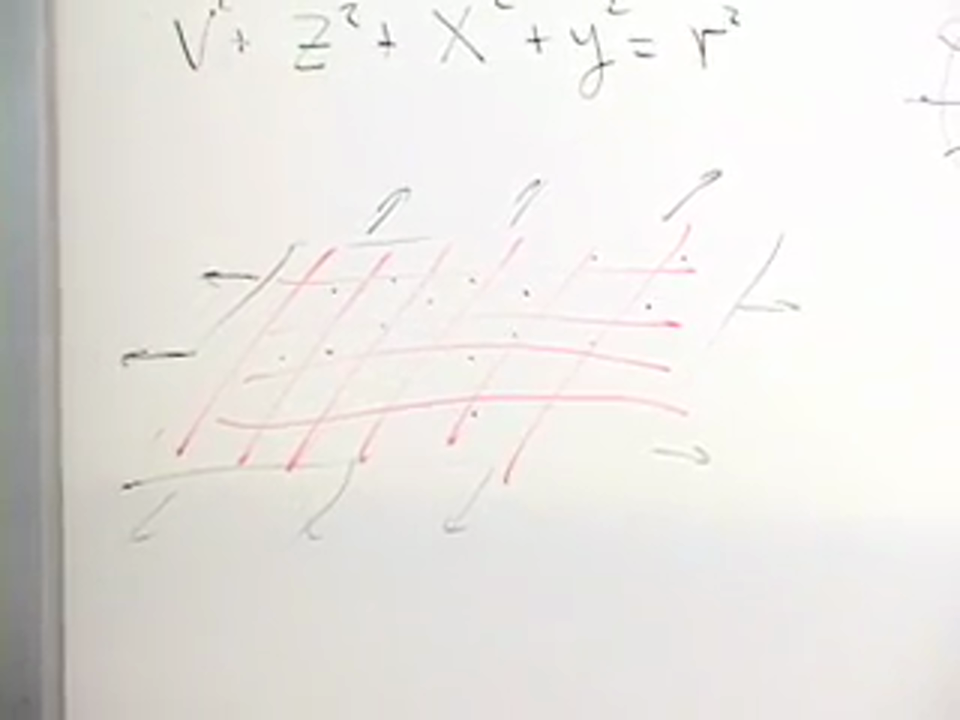
\includegraphics[width=0.72\textwidth]{lecture_09_figure_04.png}
  \caption{膨張する空間的シートに沿って運ばれる座標メッシュ。00:22:20のソースフレーム。}
  \label{fig:l09-comoving-grid-board}
\end{figure}

\(x\)軸に沿って固定された共動間隔\(\Delta x\)だけ離れた二つの物体について、それらの物理的距離は
\begin{equation}
  D(t)=a(t)\,\Delta x.
  \label{eq:l09-physical-distance}
\end{equation}
\(\Delta x\)を固定して微分すると
\begin{equation}
  v(t)=\dot a(t)\,\Delta x
      =\frac{\dot a(t)}{a(t)}D(t).
\end{equation}
次を定義すると
\begin{equation}
  H(t)\equiv\frac{\dot a(t)}{a(t)},
  \label{eq:l09-hubble-parameter}
\end{equation}
ハッブルの法則が得られる。
\begin{equation}
  v=H(t)D.
  \label{eq:l09-hubble-law}
\end{equation}
「ハッブル定数」における「定数」という語は、指定された宇宙時刻において空間全体にわたって一定であることを意味する。宇宙の歴史を通じて一定であることを意味するものではない。

\begin{figure}[H]
  \centering
  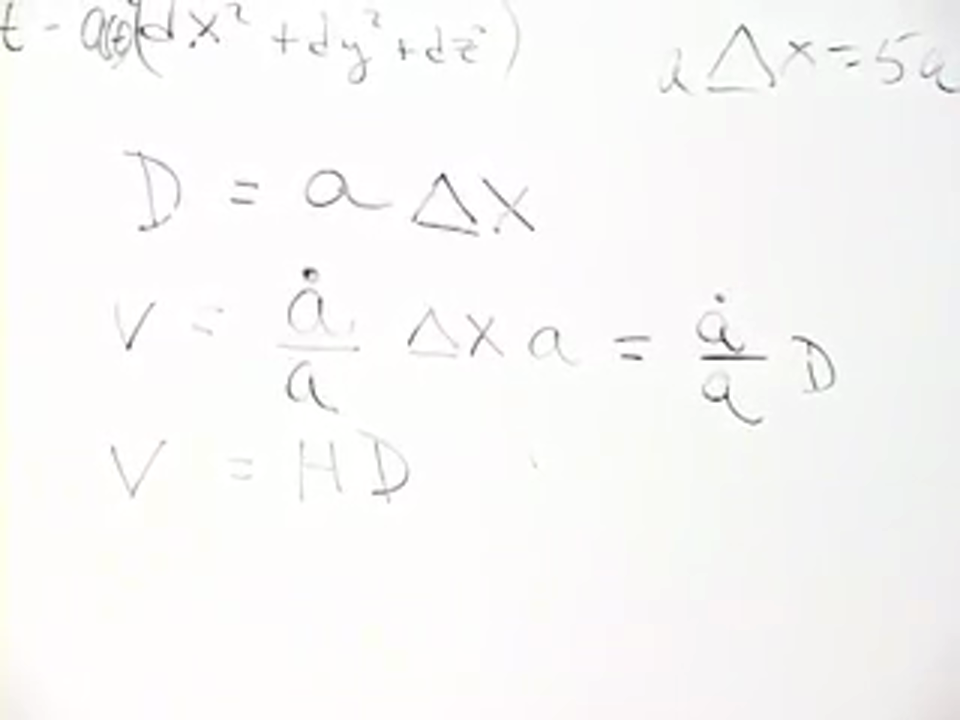
\includegraphics[width=0.72\textwidth]{lecture_09_figure_05.png}
  \caption{黒板での導出\(D=a\Delta x\)、
  \(v=(\dot a/a)D=HD\)。00:26:40のソースフレーム。}
  \label{fig:l09-hubble-board}
\end{figure}

\begin{classroomqa}
\audiencequestion{遠方の銀河がより早い時刻に見られるなら、その推定されたハッブルパラメータは本当に今日近傍で測定された値と等しいべきだろうか。}
\lecturerresponse{ルックバック時間が宇宙の年齢に比べて小さい場合に限る。適度な距離では、\(H(t)\)の変化は一つの数値が有用であるほど小さい。真に宇宙論的な距離では、我々はより早い時代を見ており、\(a\)と\(H\)の時間依存性を含めなければならない。それが、スケール因子に対する動的方程式が必要となる一つの理由である。}
\end{classroomqa}

\section{膨張する座標系におけるヌル光線}

\begin{classroomqa}
\audiencequestion{スケール因子は遠方の銀河間の光の伝播に影響するだろうか。}
\lecturerresponse{光線はヌル軌道に従うので、\(d\tau=0\)である。正の\(x\)軸に沿って進む光線では、\(dy=dz=0\)であり、膨張する計量は次を与える。
\begin{align}
  0&=dt^2-a^2(t)dx^2,
  &dt&=a(t)dx,\notag\\
  &&\frac{dx}{dt}&=\frac{1}{a(t)}.
  \label{eq:l09-null-ray}
\end{align}
座標速度は\(a(t)\)が増大するにつれて減少するが、光の局所的な物理的速度は\(c=1\)のままである。固定された座標間隔は増大する物理的距離を表す。}
\end{classroomqa}

\begin{figure}[H]
  \centering
  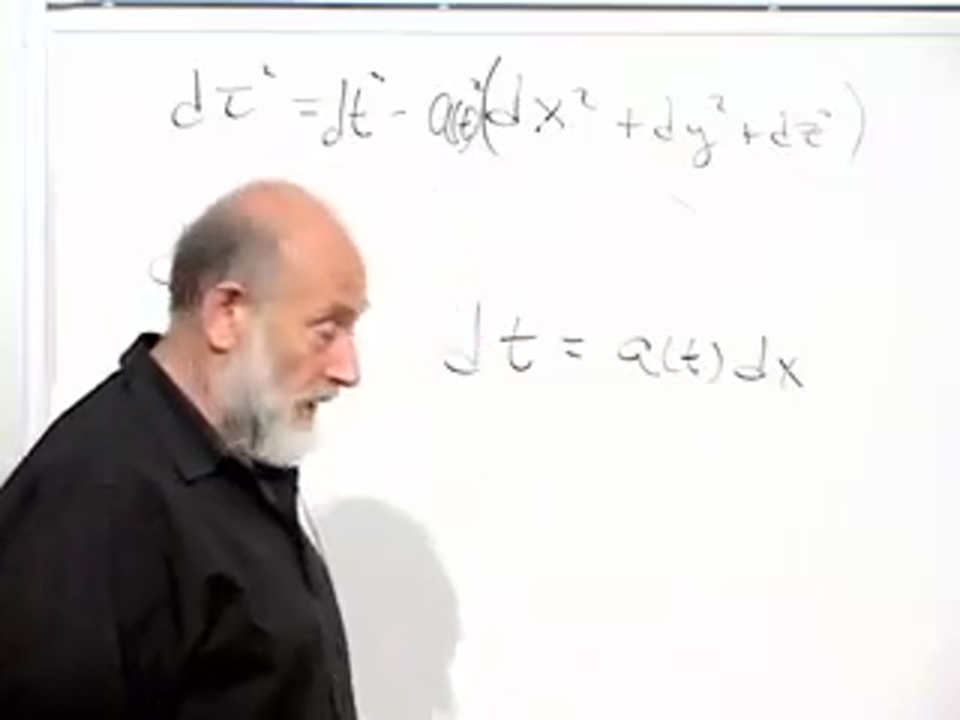
\includegraphics[width=0.72\textwidth]{lecture_09_figure_06.png}
  \caption{ヌル条件と動径方向の光伝播に対する\(dt=a(t)dx\)。00:30:54のソースフレーム。}
  \label{fig:l09-null-board}
\end{figure}

この同じ事実が「光は遠方ほど遅くなる」ように聞こえる座標を選ぶこともできるが、その場合には長さと時計がそれに対応して扱いにくい記述を帯びることになる。膨張する空間という言葉遣いの方が、自由落下するすべての観測者が同じ光速度を測定するという局所的な言明を保つので、より明快である。

\begin{classroomqa}
\audiencequestion{局所的な光の伝播と原子物理が遠方の銀河でも同じであるという証拠はあるだろうか。}
\lecturerresponse{操作的に意味があるのは無次元の比較だけである。原子の大きさを長さの単位として選び、原子的または核的な周期を時間の単位として選び、そのうえで光が選んだ長さを横切るのにそのような周期がいくつ必要かを問う。分光観測は、これらの無次元比が遠方の領域でも同じであるという言明を支持する。証拠は間接的であるが、それはまさに局所的な法則の一様性を検証する比較の一種である。}
\end{classroomqa}

観測可能な宇宙が極めて小さかったとき、光は対応する光横断単位で与えられた物理的領域を素早く横切ることができた。これは\(c\)が異なっていたことを意味しない。領域そのものが小さかったことを意味する。

\section{宇宙内部のニュートン球}

ここで運動学から力学へと移る。自分自身を原点に置き、多数の銀河と銀河団を包含するのに十分な大きさの球を描く。その境界上の銀河を一つ選ぶ。一様な宇宙では質量分布は我々のまわりで球対称であり、ニュートンの球殻定理から二つの決定的な事実が得られる：
\begin{enumerate}
  \item 選択した半径の外側にある球対称に分布した全物質は、境界の銀河に正味のニュートン力としてゼロしか及ぼさない；
  \item 球の内側にある全物質は、この動径方向の運動に対して、中心に集中しているかのように振る舞う。
\end{enumerate}
我々は静止している座標系を用いるので、以下の議論における速度と加速度は我々に対して測定される。

\begin{figure}[H]
  \centering
  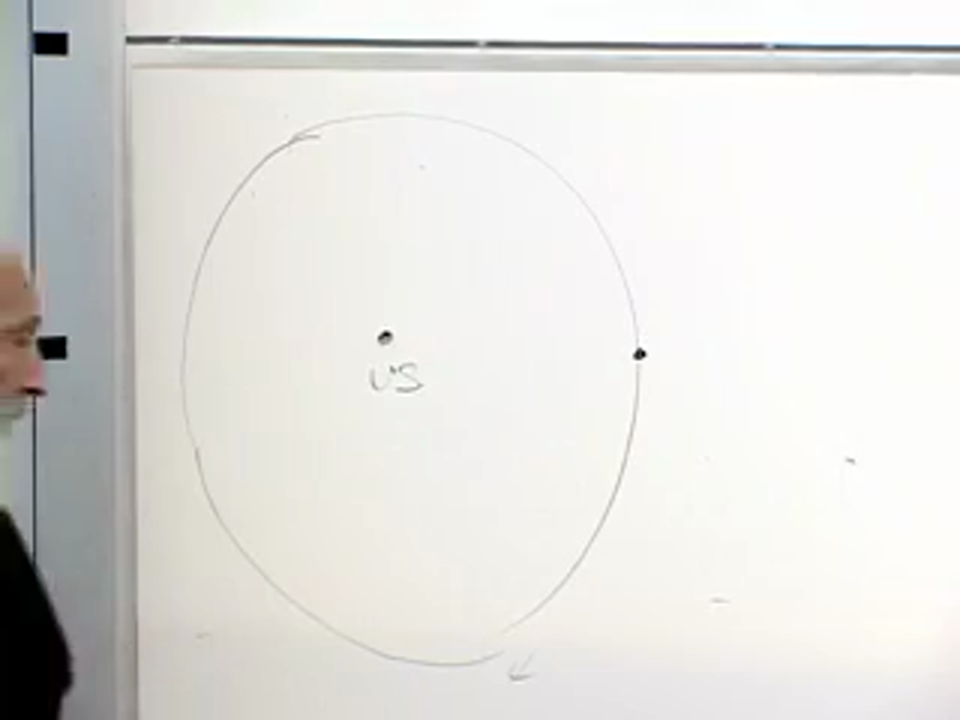
\includegraphics[width=0.72\textwidth]{lecture_09_figure_08.png}
  \caption{球殻定理の構成：我々は中心にあり、試験銀河は大きな一様球の境界上にある。00年における源フレーム：41：10。}
  \label{fig:l09-shell-board}
\end{figure}

\begin{figure}[H]
  \centering
  \begin{tikzpicture}[scale=0.92,>=Latex]
    \draw[thick] (0,0) circle (2.35);
    \fill (0,0) circle (2pt) node[below left] {us};
    \fill (2.35,0) circle (2.2pt) node[right] {test galaxy \(m\)};
    \draw[->,thick,blue!65!black] (0.18,0) -- (2.15,0)
      node[midway,above] {\(R=a(t)x\)};
    \draw[->,thick,red!65!black] (2.35,0.12) -- (3.25,0.12)
      node[midway,above] {\(v=\dot a(t)x\)};
    \node[align=center,text width=7cm] at (0,-2.85)
      {outside shells cancel;\\enclosed mass acts at the center};
  \end{tikzpicture}
  \caption{ニュートン的構成の明快な再構成。}
  \label{fig:l09-shell-clean}
\end{figure}

銀河が固定された共動座標\(x\)を持つなら、その物理的半径と速度は
\begin{equation}
  R(t)=x a(t),
  \qquad
  v(t)=x\dot a(t)=H(t)R(t).
  \label{eq:l09-radius-velocity}
\end{equation}
である。球に囲まれた質量を\(M\)、試験銀河の質量を\(m\)とする。ニュートン的エネルギーは
\begin{equation}
  E=\frac12 m v^2-\frac{GMm}{R}.
  \label{eq:l09-newtonian-energy}
\end{equation}

\begin{figure}[H]
  \centering
  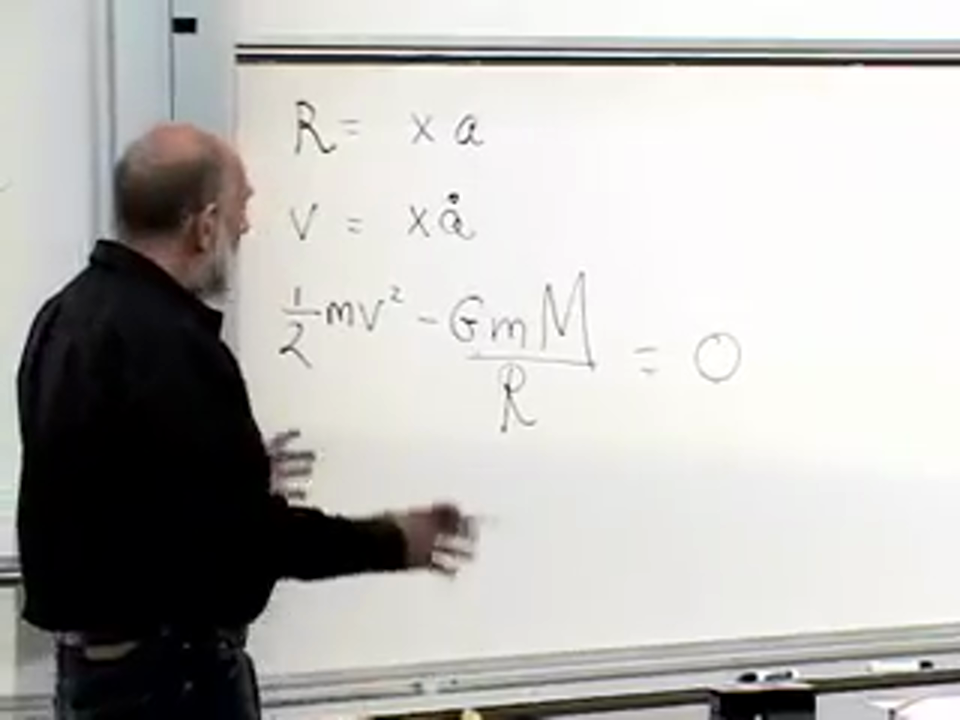
\includegraphics[width=0.72\textwidth]{lecture_09_figure_09.png}
  \caption{完全な板書の順序\(R=xa\)、\(v=x\dot a\)、および\(E=0\)に特化したニュートン的エネルギー方程式。00年における源フレーム：48：40。}
  \label{fig:l09-energy-board}
\end{figure}

エネルギーは正、ゼロ、または負であり得る。脱出と再崩壊の境界\(E=0\)から始めると、それに対して
\begin{equation}
  \frac12 v^2=\frac{GM}{R}.
  \label{eq:l09-zero-energy}
\end{equation}

\begin{classroomqa}
\audiencequestion{後退する銀河にとって全エネルギーがゼロであるとはどういう意味か？}
\lecturerresponse{それはまさに脱出速度の場合である。正のエネルギーは脱出速度を超える運動を意味し、負のエネルギーは脱出速度を下回る運動を意味し、物質のみのニュートン的描像では最終的な戻りを意味する。我々はそれらの可能性の境界から始め、平坦な方程式を導出した後に他の符号に戻る。}
\end{classroomqa}

\begin{classroomqa}
\audiencequestion{囲まれた質量\(M\)は球が膨張するにつれて変化するか？}
\lecturerresponse{いいえ。球は共動しているので、同じ粒子がその内部にとどまる。その物理的体積は増大し密度は低下するが、その全囲まれた質量は固定されたままである。\(M\)と\(\rho(t)\)のこの区別は本質的である。}
\end{classroomqa}

一様密度\(\rho(t)\)に対して、
\begin{equation}
  M=\frac{4\pi}{3}\rho(t)R^3.
  \label{eq:l09-enclosed-mass}
\end{equation}
\eqref{eq:l09-zero-energy}への代入により
\begin{equation}
  \frac12 v^2
  =\frac{G}{R}\left(\frac{4\pi}{3}\rho R^3\right).
  \label{eq:l09-enclosed-energy}
\end{equation}

\begin{figure}[H]
  \centering
  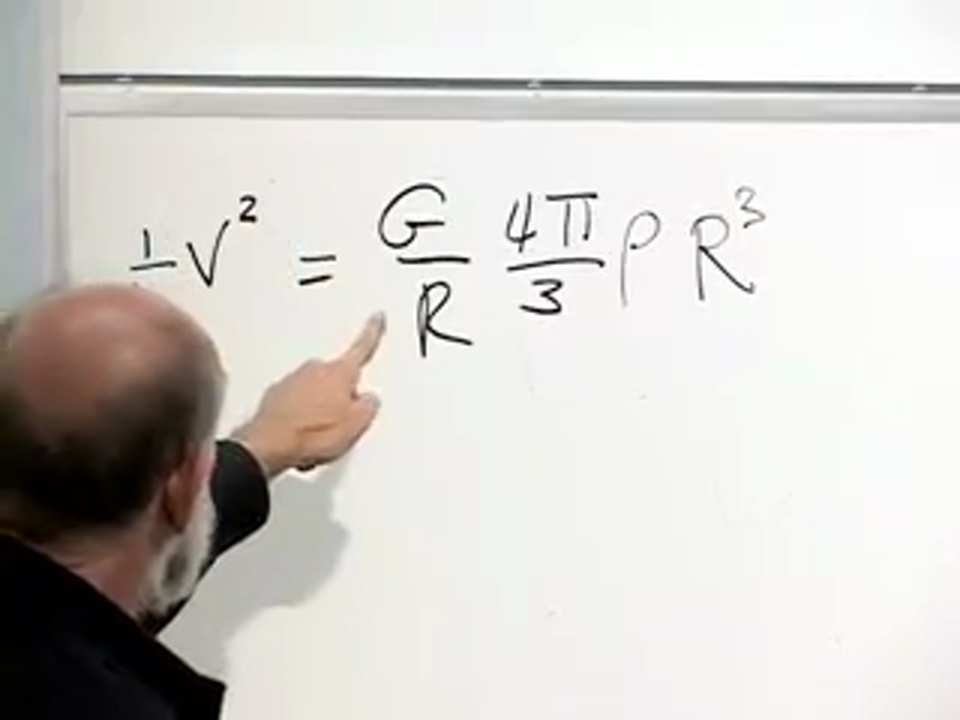
\includegraphics[width=0.72\textwidth]{lecture_09_figure_10.png}
  \caption{ゼロエネルギー方程式における囲まれた質量の代入。
  00年における源フレーム：54：16.060。}
  \label{fig:l09-enclosed-mass-board}
\end{figure}

\(v=HR\)を用いると、
\begin{align}
  \frac12 H^2R^2
    &=\frac{4\pi G}{3}\rho R^2,\\
  H^2
    &=\frac{8\pi G}{3}\rho.
\end{align}
が得られる。したがって、ゼロエネルギーで空間的に平坦な膨張則は
\begin{equation}
  \boxed{\left(\frac{\dot a}{a}\right)^2
  =\frac{8\pi G}{3}\rho(t)}.
  \label{eq:l09-flat-friedmann}
\end{equation}
である。\(R^2\)の相殺は偶然ではない。一様な宇宙は、どの共動銀河を試験対象として選んでも同じ\(H(t)\)を与えなければならない。

\begin{figure}[H]
  \centering
  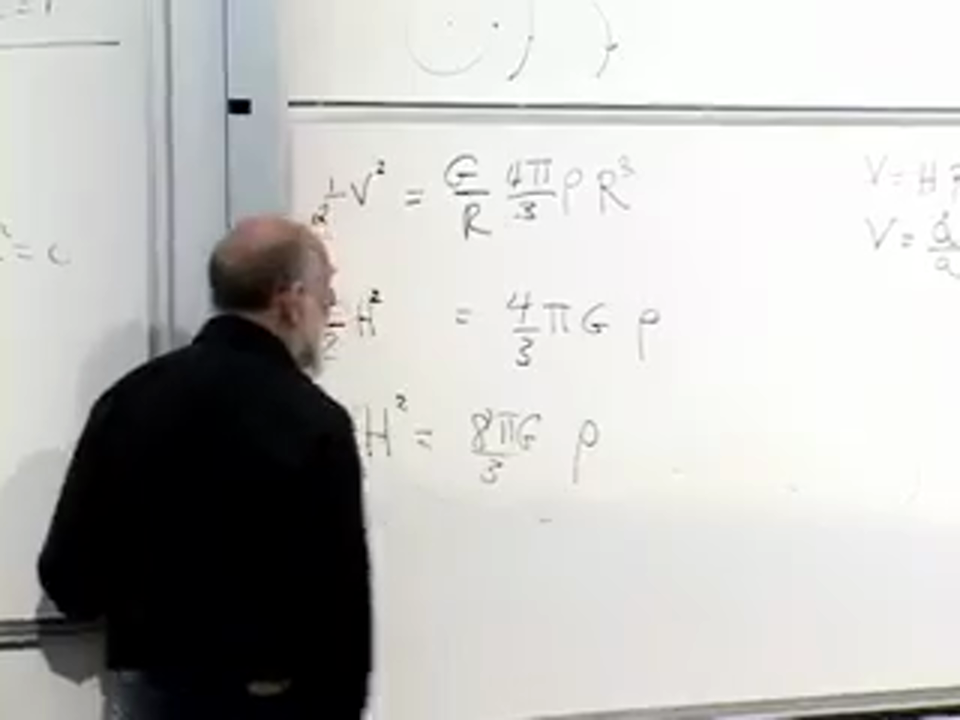
\includegraphics[width=0.72\textwidth]{lecture_09_figure_11.png}
  \caption{半径の相殺と、その結果として得られる平坦なフリードマン関係が板書に示されている。00年における源フレーム：57：30。}
  \label{fig:l09-friedmann-board}
\end{figure}

\begin{classroomqa}
\audiencequestion{ゼロエネルギー関係の証拠はあるか？}
\lecturerresponse{両辺は観測的に推論できる：\(H\)は後退データから、\(\rho\)は恒星、ガス、暗黒物質、真空エネルギーを考慮することによって。講義当時の比較では、両辺は約パーセントの精度で一致していた。この限定は重要である：すべての形態のエネルギーを含めなければならず、後の真空エネルギーの議論は素朴な脱出速度の解釈を変える。}
\end{classroomqa}

単位\(c=1\)では、質量密度とエネルギー密度は同じ単位を持つ。したがって記号\(\rho\)は、議論中の成分に適した全エネルギー密度を表す。

\section{通常の物質と3分の2の法則}

方程式\eqref{eq:l09-flat-friedmann}は、\(\rho(t)\)がどのように変化するかを知るまで閉じない。まず、共動する直方体の箱をゆっくり運動する非相対論的粒子で満たす。その座標次元は固定されているが、その物理的体積は
\begin{equation}
  V(t)=a^3(t)\,\Delta x\,\Delta y\,\Delta z.
\end{equation}
として増大する。箱の中の粒子数と静止質量は固定されたままなので、
\begin{equation}
  \rho_{\mathrm m}(t)=\frac{C_{\mathrm m}}{a^3(t)}.
  \label{eq:l09-matter-dilution}
\end{equation}
現在の時代\(t_0\)に規格化すると、
\begin{equation}
  \frac{\rho_{\mathrm m}(t)}{\rho_{\mathrm m,0}}
  =\left(\frac{a_0}{a(t)}\right)^3.
  \label{eq:l09-matter-normalized}
\end{equation}

\begin{figure}[H]
  \centering
  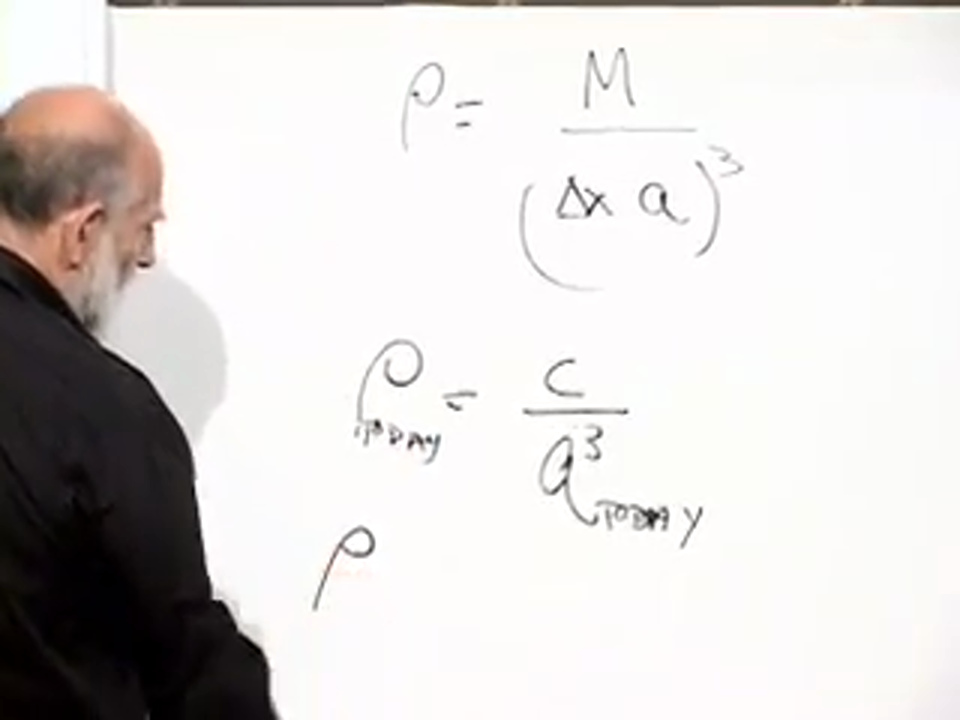
\includegraphics[width=0.72\textwidth]{lecture_09_figure_12.png}
  \caption{物質密度、その\(a^{-3}\)希釈、および現在の規格化。01年における源フレーム：04：47.940。}
  \label{fig:l09-density-board}
\end{figure}

\begin{classroomqa}
\audiencequestion{現在の宇宙の粗いエネルギー密度はどれほどで、通常の原子だけでそれを賄えるのか。}
\lecturerresponse{可視バリオン物質の数え上げでは、答えの一部しか得られない。暗黒物質と暗黒エネルギーも等価な質量エネルギーとして表さなければならない。講義では、立方メートルあたり原子一個から水素質量数十個分に及ぶ粗い尺度が引用され、精密な目録よりも桁の程度が強調されている。}
\end{classroomqa}

\eqref{eq:l09-matter-dilution}を\eqref{eq:l09-flat-friedmann}に代入し、すべての時間に依存しない因子を正の定数\(C\)に吸収すると、
\begin{equation}
  \left(\frac{\dot a}{a}\right)^2=\frac{C}{a^3},
  \qquad
  \dot a^2=\frac{C}{a}.
  \label{eq:l09-matter-ode}
\end{equation}
これを解く透明な方法が二つある。冪則の試行解\(a=K t^p\)は
\begin{equation}
  p-1=-\frac{p}{2},
  \qquad p=\frac23.
\end{equation}
を要求する。同値に、展開する平方根の分枝を取って積分すると、
\begin{equation}
  a^{1/2}\frac{da}{dt}=\sqrt C,
  \qquad
  \int a^{1/2}da=\sqrt C\int dt,
\end{equation}
となるので、時間のビッグバン起源を選んだ後、
\begin{equation}
  a^{3/2}\propto t,
  \qquad
  \boxed{a(t)\propto t^{2/3}}.
  \label{eq:l09-matter-solution}
\end{equation}
となる。ライブの導出では係数を合わせる際に一時的に因子を失うが、その後積分に戻って指数を検証する。ノートは検算を保持するが、表示するのは訂正された代数のみである。

\begin{figure}[H]
  \centering
  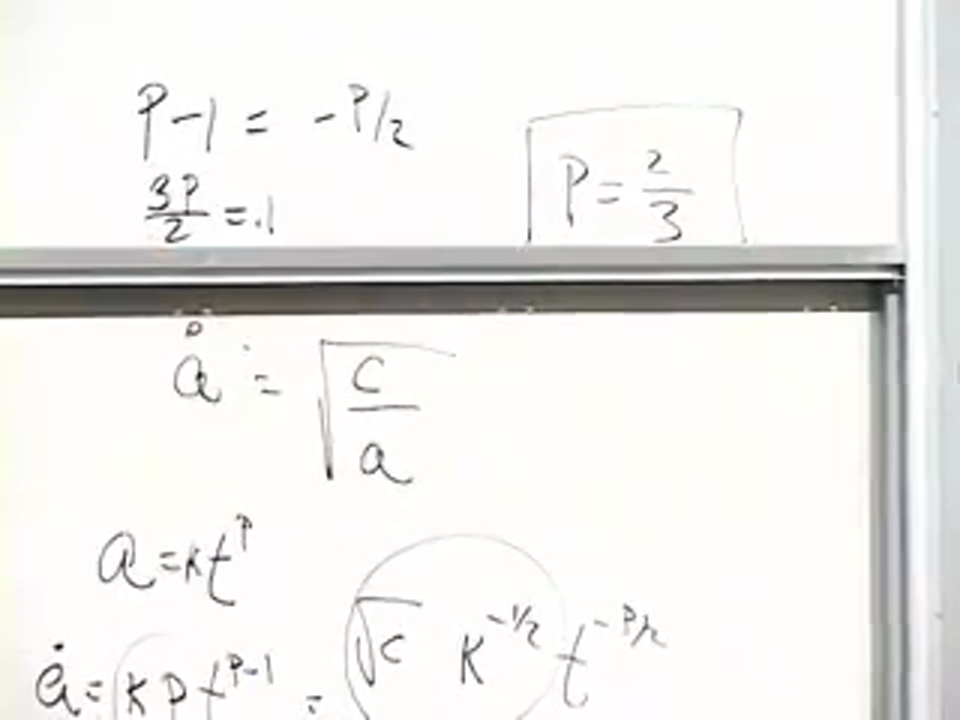
\includegraphics[width=0.72\textwidth]{lecture_09_figure_13.png}
  \caption{冪則の試行解と枠で囲まれた指数\(p=2/3\)。01のソースフレーム：13：05。}
  \label{fig:l09-matter-solution-board}
\end{figure}

解を微分すると
\begin{equation}
  H(t)=\frac{\dot a}{a}=\frac{2}{3t}.
  \label{eq:l09-matter-hubble}
\end{equation}
が得られる。ハッブルパラメータは過去においてより大きかった。したがって、無視できないルックバック時間が見えるほど遠くを見るとき、今日の\(H_0\)を変えずに局所的な線形関係を延長してはならない。

\begin{figure}[H]
  \centering
  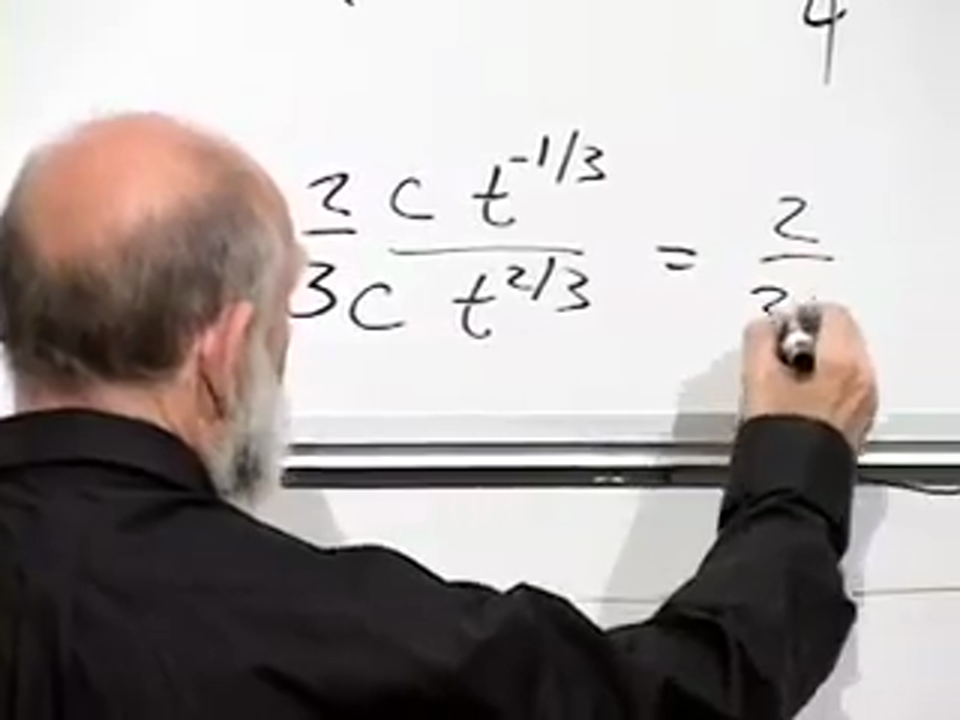
\includegraphics[width=0.72\textwidth]{lecture_09_figure_14.png}
  \caption{\(a\propto t^{2/3}\)に対して\(\dot a/a\)を取ると\(H=2/(3t)\)が得られる。01のソースフレーム：20：42。}
  \label{fig:l09-hubble-time-board}
\end{figure}

\section{エネルギーの符号と空間曲率}

ニュートン的な推論は平坦なゼロエネルギーの場合を貫いて我々を導いてきた。一般相対性理論は、球殻定理だけからは得られない事実を付け加える。ニュートン流の比エネルギーの符号は空間曲率の符号に対応する。
\begin{center}
\begin{tabular}{@{}>{\raggedright\arraybackslash}p{0.20\linewidth}
                    >{\raggedright\arraybackslash}p{0.29\linewidth}
                    >{\raggedright\arraybackslash}p{0.37\linewidth}@{}}
  \toprule
  全エネルギー & 空間曲率 & 物質のみの運命 \\
  \midrule
  正 & 負（開） & 永遠に膨張する \\
  ゼロ & ゼロ（平坦） & 脱出境界に近づく \\
  負 & 正（閉） & 膨張し、転回し、再収縮する \\
  \bottomrule
\end{tabular}
\end{center}
最後の列は真空エネルギーがないことを仮定している。発射体の類推では、正のエネルギーは脱出速度より上、ゼロはちょうど脱出速度、負は脱出速度より下を意味する。アインシュタイン方程式はこれら三つの場合をそれぞれ開いた、平坦な、閉じた空間幾何学と同一視する。

\section{光子と1/2則}

物質の法則\(\rho\propto a^{-3}\)は、各粒子のエネルギーがほぼ固定されている一方で数密度が減少すると仮定している。光子はその仮定に反する。光子に対しては、
\begin{equation}
  E=h\nu=\frac{hc}{\lambda}.
\end{equation}
膨張はその波長をスケール因子に比例して伸ばし、
\begin{equation}
  \lambda\propto a,
  \qquad E\propto a^{-1}.
\end{equation}
光子数密度は依然として\(a^{-3}\)のように減少し、各光子のエネルギーがさらに\(a^{-1}\)の因子を一つ寄与する。したがって
\begin{equation}
  \boxed{\rho_{\mathrm r}(t)\propto a^{-4}(t)}.
  \label{eq:l09-radiation-dilution}
\end{equation}

ギター弦の類推は物理的描像を捉えている。弦を弾き、次にその振動部分を長くすると、波長は長くなり音は下がる。膨張する共動箱の中の光子モードも同様に振る舞う。この描像を逆向きにたどると、圧縮は波長を短くし光子エネルギーを高める。

\begin{figure}[H]
  \centering
  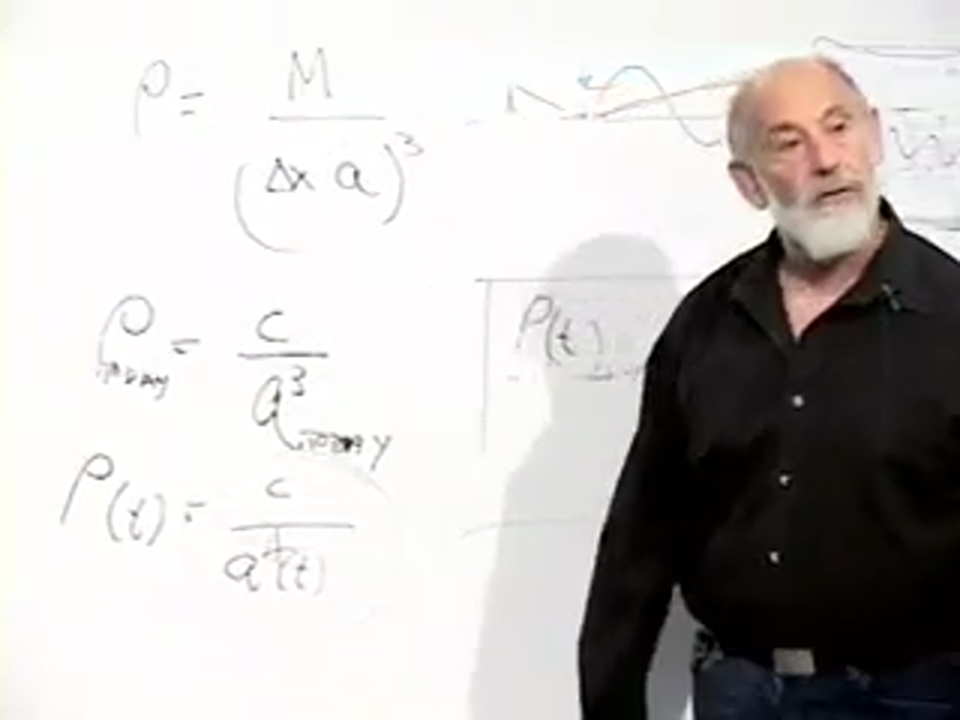
\includegraphics[width=0.72\textwidth]{lecture_09_figure_15.png}
  \caption{物質密度の関係を黒板で放射のスケーリング\(\rho_{\mathrm r}\propto a^{-4}\)へ拡張したもの。01のソースフレーム：29：20。}
  \label{fig:l09-radiation-board}
\end{figure}

平坦なフリードマン方程式で\(\rho_{\mathrm r}\propto a^{-4}\)を用いると
\begin{equation}
  \left(\frac{\dot a}{a}\right)^2=\frac{C_{\mathrm r}}{a^4},
  \qquad
  \dot a\propto a^{-1},
\end{equation}
が得られ、したがって
\begin{equation}
  \boxed{a(t)\propto t^{1/2}}.
  \label{eq:l09-radiation-solution}
\end{equation}
となる。これは\(t^{2/3}\)よりゆっくり成長する。十分に過去へさかのぼると、\(a\)が減少するにつれて\(a^{-4}\)が\(a^{-3}\)より速く上昇するため、放射が通常の物質を支配しなければならない。講義では物質と放射の交差を、スケール因子が今日よりおよそ千倍小さかった時代のあたりに置いている。その交差より前、宇宙は放射支配であり、その後、長い期間にわたって物質支配であった。

\section{真空エネルギーと指数関数的膨張}

真空エネルギーは逆のスケーリング挙動を示す。その密度は空の空間の性質であり、宇宙が膨張しても薄まらない：
\begin{equation}
  \rho_\Lambda=\text{constant}.
  \label{eq:l09-vacuum-density}
\end{equation}
通常の物質と放射は過去に向かってより密になるが、この項はそうならない。したがって初期宇宙ではより重要でなく、他の成分が薄まるにつれてより重要になる。講義では、真空エネルギーが今日の宇宙エネルギー密度のおよそ\(70\%\)を供給するという当時の推定を用いている。

\(\rho_\Lambda\) を一定とすると、式 \eqref{eq:l09-flat-friedmann} は一定の膨張率を与える。
\begin{equation}
  H_\Lambda=\sqrt{\frac{8\pi G}{3}\rho_\Lambda},
  \qquad
  \frac{\dot a}{a}=H_\Lambda.
\end{equation}
したがって
\begin{equation}
  \boxed{a(t)=a(t_i)e^{H_\Lambda(t-t_i)}}.
  \label{eq:l09-vacuum-solution}
\end{equation}

\begin{figure}[H]
  \centering
  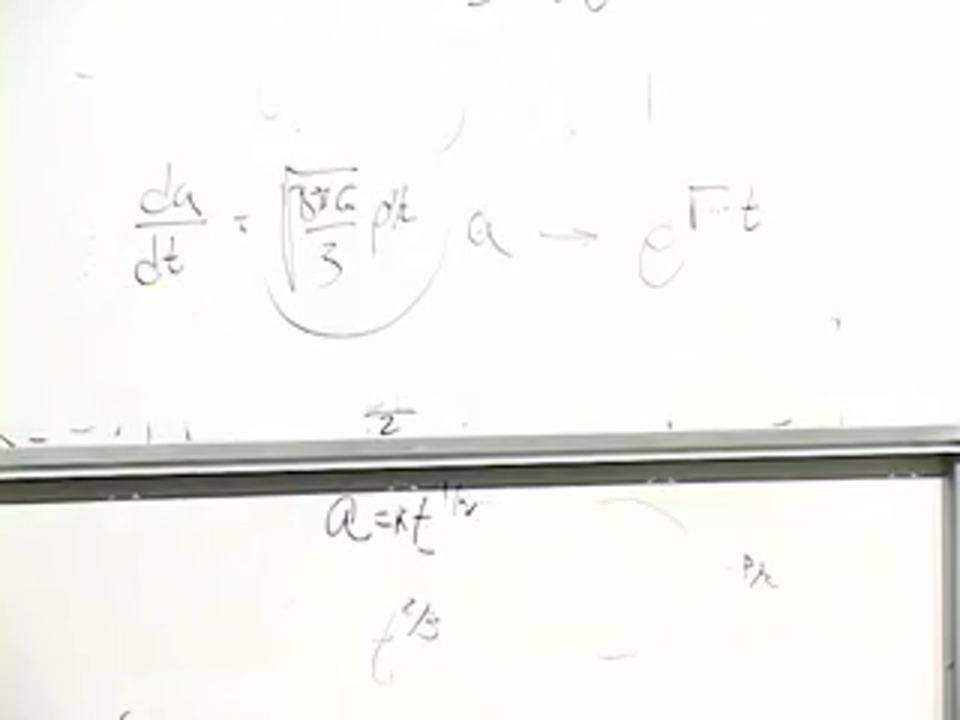
\includegraphics[width=0.72\textwidth]{lecture_09_figure_16.png}
  \caption{指数関数的膨張を導く定数密度の式。
  ソースフレーム 01:35:48。}
  \label{fig:l09-vacuum-board}
\end{figure}

講義で引用された観測スケールでは、宇宙の線形サイズはおよそ百億年から百二十億年で二倍になる。この小さく非零の真空密度の起源は依然として説明されていない。その存在と膨張への影響は経験的事実である。

\begin{classroomqa}
\audiencequestion{この議論において、真空エネルギーはダークエネルギーと同じものか。}
\lecturerresponse{はい。ここで「ダークエネルギー」とは一定の真空エネルギー密度、等価的には宇宙定数を指す。より一般的な時間依存ダークエネルギーモデルも想像できるが、それらはこの講義の計算の一部ではない。}
\end{classroomqa}

\section{膨張する宇宙が光を赤方偏移させる仕組み}

\begin{classroomqa}
\audiencequestion{光子は、我々が膨張する共動座標を選んだこと、したがって光子がエネルギーを下げることを、どうして知り得るのか。}
\lecturerresponse{光子は我々のラベルに反応しない。光子は、物理的間隔が変化する幾何学の中を伝播する。物理的サイズが二倍になる領域を占める波連は、二倍の波長を獲得する。共動座標はこの伸張を簡潔に記述するにすぎず、それを引き起こすのではない。}
\end{classroomqa}

\begin{classroomqa}
\audiencequestion{今日我々に到達する背景光子はどこから来るのか。}
\lecturerresponse{より遠くを見ることはより昔を見ることである。やがて我々は、宇宙の物質が電離プラズマであった時代を見る。それは自由な荷電粒子によって光子が繰り返し散乱されるため不透明である。光子が最後に自由に我々へと旅することができた境界は、観測者を取り囲む球として現れる。すなわち最終散乱面である。}
\end{classroomqa}

\begin{figure}[H]
  \centering
  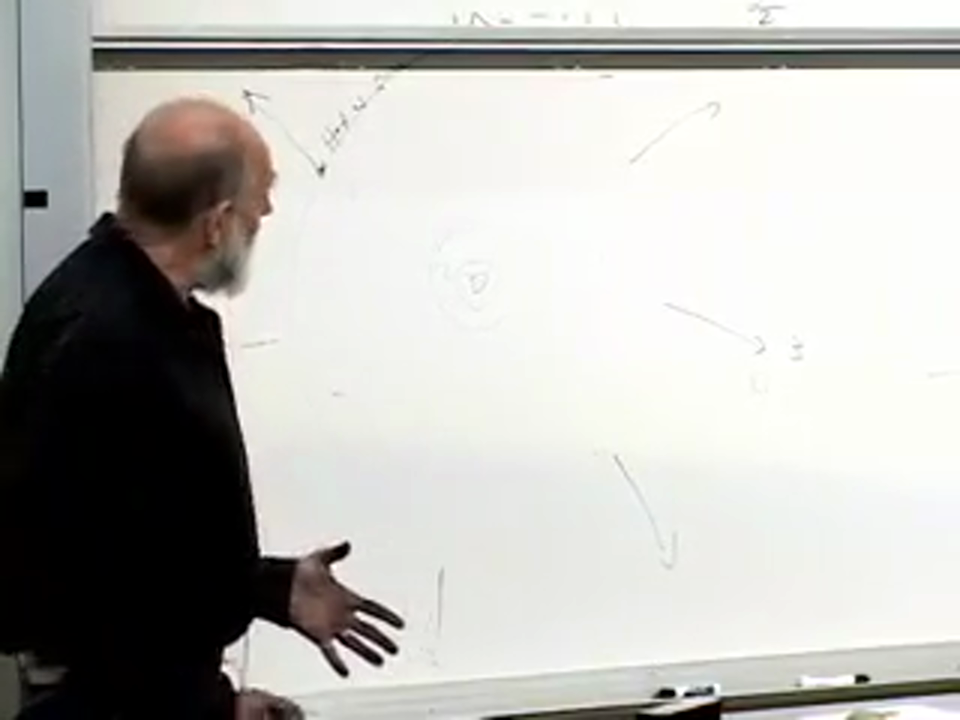
\includegraphics[width=0.72\textwidth]{lecture_09_figure_17.png}
  \caption{最終散乱面と次第に遠くなる殻の観測者中心のスケッチ。ソースフレーム 01:42:05。}
  \label{fig:l09-last-scattering-board}
\end{figure}

\begin{figure}[H]
  \centering
  \begin{tikzpicture}[scale=0.9,>=Latex]
    \fill (0,0) circle (2pt) node[below] {observer};
    \draw[thick,orange!70!black] (0,0) circle (2.55);
    \node[orange!70!black,align=center] at (0,3.05)
      {surface of last scattering};
    \foreach \a in {25,75,145,210,285,335}{
      \draw[->,blue!60!black] ({2.55*cos(\a)},{2.55*sin(\a)}) --
        ({1.7*cos(\a)},{1.7*sin(\a)});
    }
    \draw[decorate,decoration={snake,amplitude=1.5pt,segment length=7pt},
      red!65!black,thick,->] (-2.5,0) -- (-0.15,0);
    \node[red!65!black,below] at (-1.35,-0.15)
      {redshifted photon};
  \end{tikzpicture}
  \caption{最終散乱の描像の明瞭な再構成。}
  \label{fig:l09-last-scattering-clean}
\end{figure}

その放射は高温プラズマに特徴的なスペクトルで放出され、およそ千倍長い波長で我々に到達する。講義のドップラー的表現では、遠方の放射面は速やかに後退し、その放射は強く赤方偏移する。幾何学的表現では、波は伝播の間に伸張する。両方の描像は同じ関係を表しており、\begin{equation}
  1+z=\frac{\lambda_0}{\lambda_{\mathrm{em}}}
      =\frac{a_0}{a_{\mathrm{em}}}.
  \label{eq:l09-cosmological-redshift}
\end{equation}
\editorialnote{式\eqref{eq:l09-cosmological-redshift}は、講義の伸張およびドップラーによる記述の標準的な定量的形式である。}

より早い観測時代には、最終散乱球は対応する描像においてより近くにあり、観測される背景光子はより赤方偏移が小さく、したがってより高エネルギーであったであろう。宇宙時間が進むにつれて、その初期プラズマから共動観測者に到達する光子は次第に長い波長を持つ。

\section{赤方偏移した光子のエネルギーはどこへ行くのか。}

\begin{classroomqa}
\audiencequestion{光子はエネルギー \(h\nu_{\mathrm{em}}\) で放出され、より少ないエネルギーで赤方偏移して到達する。その差はどうなったのか。}
\lecturerresponse{ニュートン的導出はエネルギー方程式として始まった。その宇宙論的形式は膨張率を物質エネルギー密度に関係づけるので、物質エネルギーと膨張を別々に保存される会計として扱うことはできない。講義は、失われた光子エネルギーが膨張の運動学的な帳簿に入ると記述する。放射で満たされたピストンがこの類推を具体的にする。放射圧がピストンを外側へ押し、光子の波長が増大し、失われたエネルギーが力学的仕事とピストンの運動エネルギーになる。}
\end{classroomqa}

\begin{figure}[H]
  \centering
  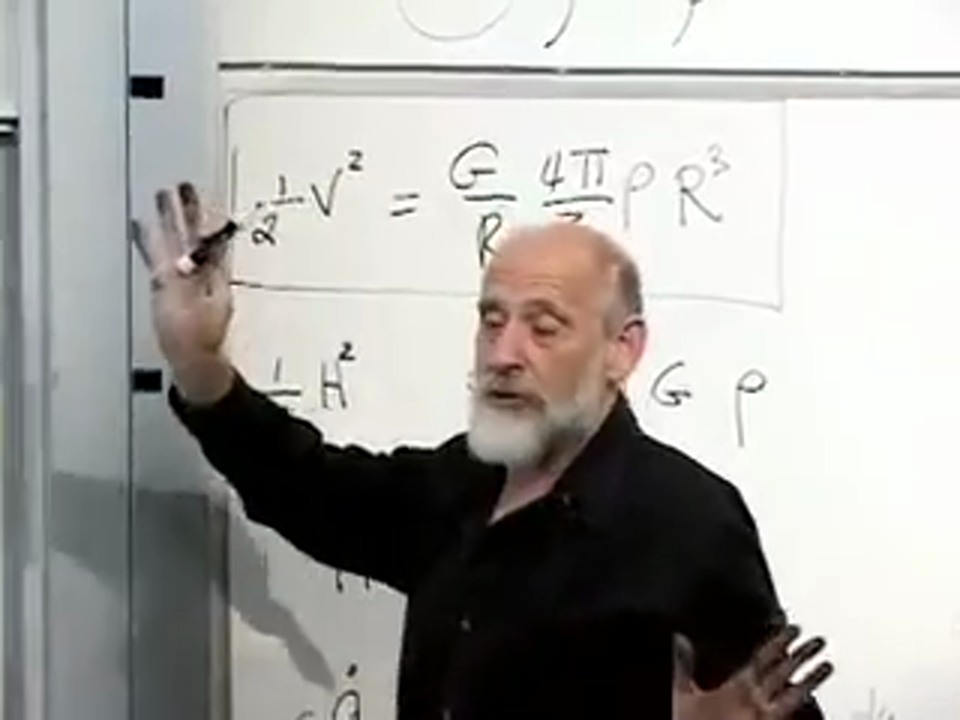
\includegraphics[width=0.72\textwidth]{lecture_09_figure_18.png}
  \caption{黒板は、枠で囲まれたニュートン的エネルギー方程式を対応するフリードマン方程式の上に置いている。ソースフレーム 01:44:42。}
  \label{fig:l09-energy-bookkeeping-board}
\end{figure}

\begin{classroomqa}
\audiencequestion{何が放射エネルギーを膨張に結合するのか。}
\lecturerresponse{圧力である。可動ピストンを備えたシリンダーでは、光子が壁に運動量を移す。ピストンが動くにつれて、放射は仕事をし、その波長は増大し、そのエネルギーは減少する。一様に膨張する宇宙には文字通りの外側のピストンはないが、\(p\,dV\) の類推は、放射のエネルギー密度が単なる数密度の希釈よりも速く減少する理由を説明する。}
\end{classroomqa}

\begin{figure}[H]
  \centering
  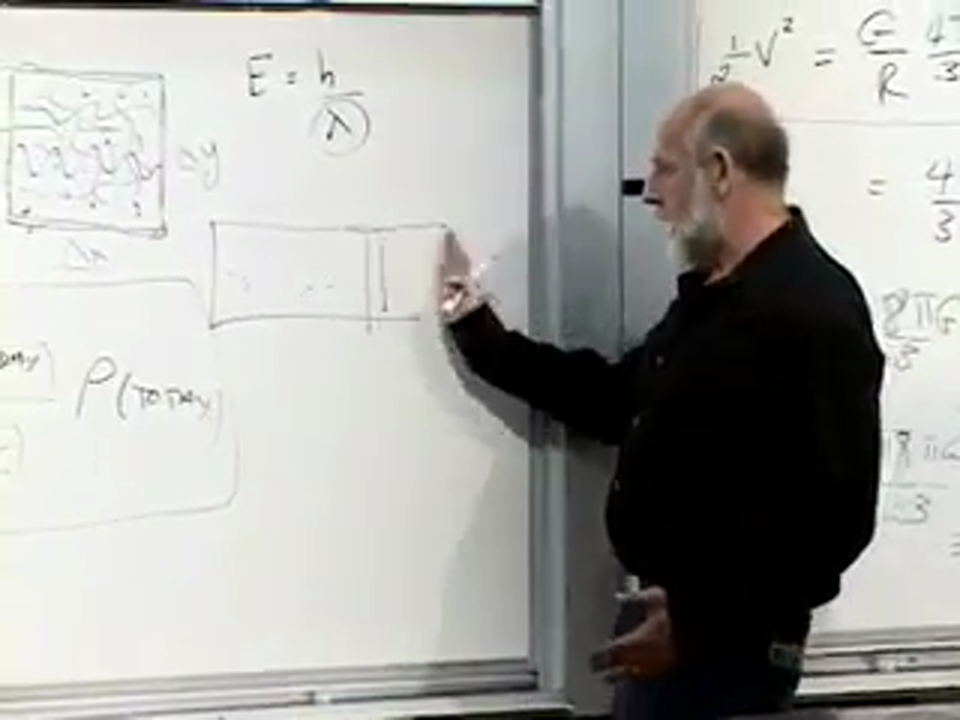
\includegraphics[width=0.72\textwidth]{lecture_09_figure_19.png}
  \caption{圧力仕事を可視化するために用いられる、可動の光子で満たされたピストン。ソースフレーム 01:46:40。}
  \label{fig:l09-piston-board}
\end{figure}

\begin{figure}[H]
  \centering
  \begin{tikzpicture}[scale=0.92,>=Latex]
    \draw[thick] (0,0) rectangle (5.3,2.6);
    \draw[very thick] (4.25,0) -- (4.25,2.6);
    \draw[very thick] (4.25,1.3) -- (5.25,1.3);
    \draw[->,thick,red!65!black] (5.25,1.3) -- (6.2,1.3)
      node[right] {moving piston};
    \foreach \y in {0.55,1.3,2.05}{
      \draw[decorate,decoration={snake,amplitude=1.4pt,segment length=6pt},
        blue!65!black,->] (0.35,\y) -- (3.9,\y);
    }
    \node at (2.15,-0.45) {radiation does \(p\,dV\) work};
  \end{tikzpicture}
  \caption{放射ピストンの類推の整理された再構成。}
  \label{fig:l09-piston-clean}
\end{figure}

一般相対性理論におけるエネルギーには注意が必要である。一般的な膨張時空では、孤立したニュートン系のエネルギーに相当する、一意に保存される大域的なエネルギーが存在する必要はない。局所的な応力エネルギーの保存は依然として成り立ち、一様な流体に対しては連続の式
\begin{equation}
  \dot\rho+3H(\rho+p)=0,
  \label{eq:l09-continuity}
\end{equation}
が得られる。この式には、物質と放射のスケーリング則の背後にある圧力仕事の項が含まれている。\editorialnote{式\eqref{eq:l09-continuity}は、講義で意図的にニュートン的なエネルギー収支の類推の基礎となっている、正確な局所的一般相対論的表現である。}

真空エネルギーはこの難問を特に鋭くする。その密度は体積が増大しても一定に保たれるため、共動領域内の全真空エネルギーは増加する。その負の圧力は重力源の一部であり、加速膨張を駆動する。したがって、幾何学と圧力仕事を含めずに、素朴な「共動箱の中の物質エネルギー」の独立した保存を要求すべきではない。

\section{なぜスケール因子を時間項から除くことができるのか}

\begin{classroomqa}
\audiencequestion{なぜスケール因子は計量の空間部分には掛かるが、時間部分には掛からないのか。}
\lecturerresponse{それは時間座標の選び方である。共形時間座標\(t\)から出発し、
\begin{equation}
  d\tau^2=A^2(t)\left(dt^2-dx^2\right).
\end{equation}
とする。新しい宇宙時間\(T\)を
\begin{equation}
  dT=A(t)\,dt.
\end{equation}
によって定義する。すると
\begin{equation}
  d\tau^2=dT^2-A^2\bigl(t(T)\bigr)dx^2.
\end{equation}
となる。時間微分の前の共通因子は消え、物理的なスケール因子は空間項に残る。}
\end{classroomqa}

\begin{figure}[H]
  \centering
  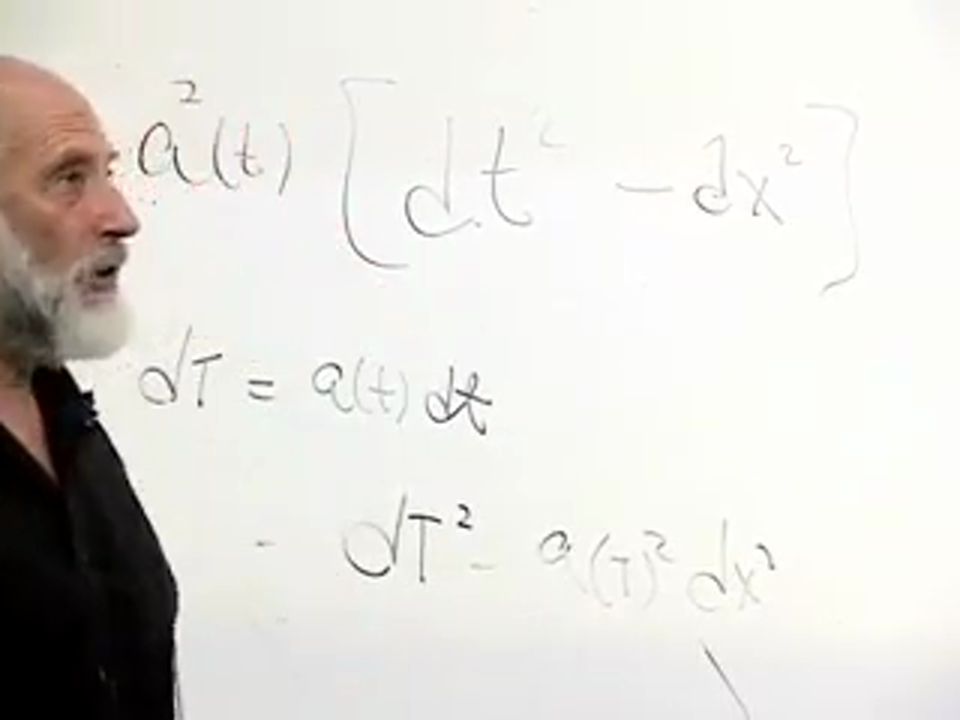
\includegraphics[width=0.72\textwidth]{lecture_09_figure_20.png}
  \caption{共形時間を宇宙時間に変換する時間の再定義\(dT=A(t)dt\)。01におけるソースフレーム：51：05。}
  \label{fig:l09-time-reparam-board}
\end{figure}

\section{曲率、真空エネルギー、宇宙の運命}

\begin{classroomqa}
\audiencequestion{もし宇宙が正の曲率を持っていたなら、銀河が我々に向かって来るのをすでに見るべきではないか。}
\lecturerresponse{必ずしもそうではない。脱出速度を下回る速度で打ち上げられた物体は、まず外側へ進み、転回点に達し、その後になって初めて落下して戻る。我々は宇宙を膨張段階で観測している。真空エネルギーがなければ、正の曲率を持つ物質宇宙は最終的に再収縮するであろう。十分に大きな正の真空エネルギーはその転回を妨げ、観測値は、小さな空間曲率にかかわらず長期的な膨張を指数的にするのに十分な大きさであるように見える。}
\end{classroomqa}

指数的な未来はエネルギーの楽園ではない。恒星は最終的に燃え尽き、物質と放射の密度は指数的に減少し、遠方の領域は因果的接触の外へと去っていく。真空エネルギーは残るが、通常の構造は次第に冷たく希薄になっていく。

\begin{classroomqa}
\audiencequestion{さらに過去を見ると、通常の粒子よりも光子の方が多いのか。}
\lecturerresponse{光子とバリオンの数比はすでに膨大であり、講義の見積もりではバリオンあたりおよそ\(10^{10}\)個の光子であり、共動体積中の両方の数はほぼ一定に保たれる。過去に向かって変化するのは主に光子あたりのエネルギーである。光子のエネルギーは\(a^{-1}\)として上昇するが、非相対論的な静止質量はそうではない。したがって、数比自体は変化する必要がないにもかかわらず、初期には放射がエネルギー密度を支配する。}
\end{classroomqa}

中心的な教訓は、幾何学だけでは宇宙の歴史は決まらないということである。平坦なフリードマン方程式は膨張とエネルギー密度の関係を与えるが、物質の内容が時間依存性を与える。非相対論的物質は\(a\propto t^{2/3}\)を与え、放射は\(a\propto t^{1/2}\)を与え、一定の真空エネルギーは指数的膨張を与える。これら三つの法則が宇宙の successive な時代を組織し、同じスケール因子が距離、赤方偏移、変化するハッブルパラメータを支配する理由を説明する。
